
\section{introduction}

\begin{frame}{slogans \& scope}

slogans:
  \begin{itemize}
  \item \alert{focus on approximating ice flow}
  \item \alert{example numerical codes that actually work}
  \end{itemize}
\medskip

scope:
  \begin{itemize}
  \item[$\circ$] continuum models

    \begin{itemize}
    \item shallow ice approximation (SIA) in 2D
    \item shallow shelf approximation (SSA) in 1D
    \item mass continuity \& surface kinematical equations
    \end{itemize}

  \item[$\circ$] numerical ideas

    \begin{itemize}
    \item finite difference schemes
    \item solving algebraic systems from stress balances
    \item verification
    \end{itemize}
  \end{itemize}
\medskip

notation: see printed notes
\end{frame}


\begin{frame}{outside of scope}

\large\emph{not} \normalsize covered here:\normalsize
\medskip

  \begin{itemize}
  \item Stokes and ``higher order'' flow equations
  \item thermomechanical coupling or polythermal ice
  \item subglacial hydrology/processes
  \item mass balance and snow/firn processes
  \item constitutive relations other than Glen isotropic
  \item grounding lines, calving fronts, ocean interaction
  \item paleo-climate and ``spin-up''
  \item earth deformation under ice sheet load
  \item other numerics: FEM, spectral, multigrid, parallel, \dots
  \item etc.
  \end{itemize}

\end{frame}


\begin{frame}{Matlab/Octave codes}

\begin{itemize}
\item lectures are structured around 16 Matlab codes
\item they also work in Octave
\item each is 1/2 to one page
\item \texttt{.zip} and \texttt{.tar.gz} forms available from memory stick
\item online:

\bigskip\bigskip\small
\centerline{\fbox{\url{http://www.dms.uaf.edu/~bueler/karthaus/}}}
\end{itemize}
\end{frame}


\subsection{ice flow equations}

\begin{frame}{my goal for the first hour}

\begin{itemize}
\item my goal is to get to an equation for which I can say:
\bigskip

\begin{center}
\emph{numerically solve just this equation, and you've got a usable model for a flowing ice sheet}
\end{center}
\bigskip

\item a ``usable'' model is \emph{understood} more than it is \emph{correct}
\item to get to my goal I will quickly recall some continuum mechanics
\end{itemize}
\end{frame}


\begin{frame}{ice in glaciers is a \emph{fluid}}

\begin{itemize}
\item we describe fluids primarily by a \emph{velocity field} $\mathbf{u}(t,x,y,z)$
\item if the ice fluid were
  \begin{itemize}
  \item[$\circ$] faster-moving than it actually is, and
  \item[$\circ$] linearly-viscous like liquid water
  \end{itemize}
  
  then ice flow would be a ``typical'' fluid
\item we would use the Navier-Stokes equations as our flow model:
\begin{align*}
\nabla \cdot \mathbf{u} &= 0 &&\text{\emph{incompressibility}} \\
\rho \left(\mathbf{u}_t + \mathbf{u}\cdot\nabla \mathbf{u}\right) &= -\nabla p + \nu \nabla^2 \mathbf{u} + \rho \mathbf{g} &&\text{\emph{force balance}}
\end{align*}
\item so, to numerically model our fluid, we grab a textbook on ``computational fluid dynamics''
\item right?
\end{itemize}
\end{frame}


\begin{frame}{\emph{hmmm} \dots \emph{does not sound like glaciology to me!}}

is numerical ice flow modeling a part of computational fluid dynamics?

\begin{itemize}
\item \alert{yes}
\item large scale like atmosphere/ocean
\item \dots but it is a weird one
\item consider what makes atmosphere/ocean flow modeling exciting:
  \begin{itemize}
  \item[$\circ$] turbulence
  \item[$\circ$] convection
  \item[$\circ$] coriolis force
  \item[$\circ$] density variation
  \item[$\circ$] chemistry (methane, ozone, \dots)
  \end{itemize}
\item none of the above is very relevant to ice flow
\item so what could be interesting about the flow of slow, cold, stiff, laminar, inert old ice?

 \qquad \dots \qquad it's \emph{ice dynamics!}
\end{itemize}
\end{frame}


\begin{frame}{ice is a slow, shear-thinning fluid}

\begin{itemize}
\item our fluid is

  \begin{tabular}{lc}
  \emph{slow}: & $\rho \left(\mathbf{u}_t + \mathbf{u}\cdot\nabla \mathbf{u}\right) \approx 0$ \\
  \emph{non-Newtonian}: & viscosity $\nu$ is not constant
  \end{tabular}
\item ``slow'':
  $$\rho \left(\mathbf{u}_t + \mathbf{u}\cdot\nabla \mathbf{u}\right) \approx 0 \qquad \iff \qquad \begin{pmatrix} \text{forces of inertia} \\ \text{are negligible} \end{pmatrix}$$
\item ``non-Newtonian'' flow:  it is ``shear-thinning'', so larger strain rate means smaller viscosity
\item so the standard ice flow model is Glen-law ($n=3$) Stokes:
\begin{align*}
\nabla \cdot \mathbf{u} &= 0 &&\text{\emph{incompressibility}} \\
0 &= - \nabla p + \nabla \cdot \tau_{ij} + \rho \mathbf{g} &&\text{\emph{force balance}} \\
\mathbf{D}u_{ij} &= A \tau^2 \tau_{ij} &&\text{\emph{flow law}}
\end{align*}
\end{itemize}
\end{frame}


\begin{frame}{ice is a slow fluid 2}

\begin{itemize}
\item equations on previous slide are true at every instant
\item
  \begin{quote}
  \alert{geometry, boundary stress, and ice viscosity determine velocity field instantaneously}
  \end{quote}
\item a time-stepping ice sheet code recomputes the velocity field at every time step, without requiring velocity from the previous step\footnote{to be a weatherman you've got to know which way the wind blows \dots but don't expect that from a glaciologist}
\item thus no memory of previous momentum/velocity, so velocity is a ``diagnostic'' output of an ice flow model
\end{itemize}
\end{frame}


\begin{frame}{plane flow Stokes}

\begin{itemize}
\item in the $x,z$ plane flow case the Stokes equations say
\begin{empheq}[]{align}
u_x + w_z &= 0 &&\text{\emph{incompressibility}}\notag \\
p_x &= \tau_{11,x} + \tau_{13,z} &&\text{\emph{stress balance} ($x$)} \notag \\
p_z &= \tau_{13,x} - \tau_{11,z} - \rho g &&\text{\emph{stress balance} ($z$)} \notag \\
u_x &= A \tau^2 \tau_{11} &&\text{\emph{flow law} (diagonal)}\notag \\
u_z + w _x &= 2 A \tau^2 \tau_{13} &&\text{\emph{flow law} (off-diagonal)} \notag
\end{empheq}
\item $x,z$ subscripts are partial derivatives
\item $\tau_{13}$ is a ``vertical'' shear stress
\item $\tau_{11}$ and $\tau_{33}=-\tau_{11}$ are deviatoric longitudinal stresses 
\item we have five equations in five unknowns ($u,w,p,\tau_{11},\tau_{13}$)
\item complicated enough \dots
\item what about in a simplified situation?
\end{itemize}
\end{frame}


\subsection{slab-on-a-slope}

\begin{frame}{slab-on-a-slope}

\vspace{-0.05in}
\small

\begin{columns}

\begin{column}{0.5\textwidth}
\begin{itemize}
\item rotated coordinates:
  $$\mathbf{g} = g \sin\alpha\, \hat x - g \cos \alpha \,\hat z$$
\item so $p_x,p_z$ equations are now:
\begin{align}
p_x &= \tau_{11,x} + \tau_{13,z} + \rho g \sin\alpha \notag \\
p_z &= \tau_{13,x} - \tau_{11,z} - \rho g \cos\alpha \notag
\end{align}
\end{itemize}
\end{column}

\begin{column}{0.5\textwidth}
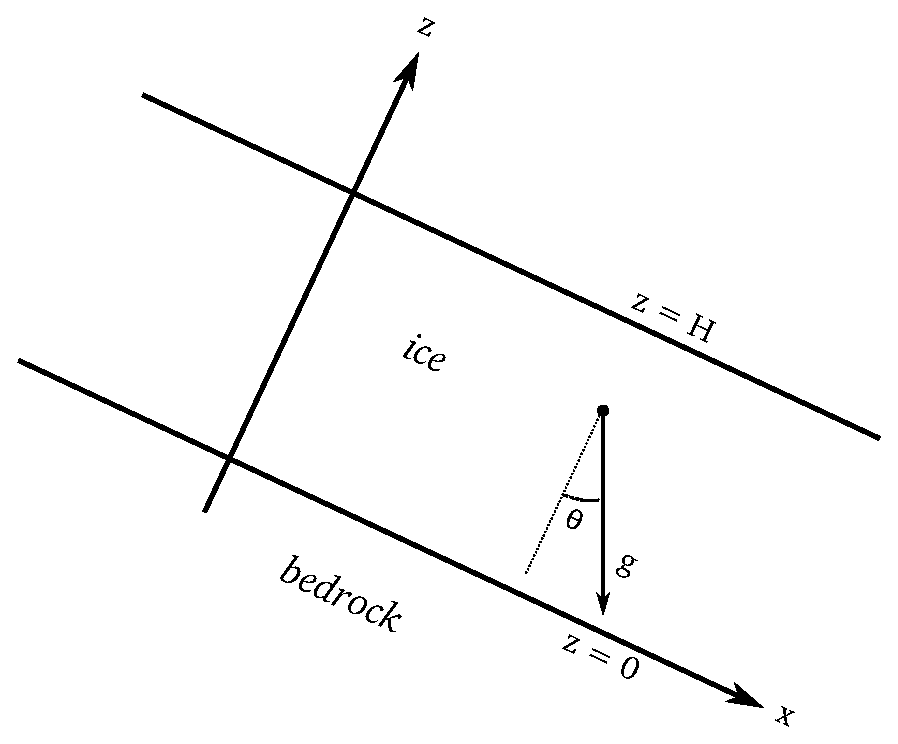
\includegraphics[width=1.0\textwidth]{slab}
\end{column}

\end{columns}

\begin{itemize}
\item for a slab-on-a-slope there is \emph{no variation in} $x$
\item so equations simplify:
\small
\begin{empheq}[box=\fbox]{align}
w_z &= 0 &   0 &= \tau_{11} \notag \\
\tau_{13,z} &= - \rho g \sin\alpha &   u_z &= 2 A \tau^2 \tau_{13} \notag \\
p_z &= - \rho g \cos\alpha \notag
\end{empheq}
\normalsize
\end{itemize}
\end{frame}


\begin{frame}{slab-on-a-slope 2}

\begin{itemize}
\item add some boundary conditions:
	$$w(\text{base})=0, \qquad p(\text{surface})=0, \qquad u(\text{base})=u_0$$
\item by integrating vertically, get :
  $$w=0, \qquad p = \rho g \cos\alpha (H-z), \qquad \tau_{13} = \rho g \sin\alpha (H-z)$$
\item and from ``$u_z = 2 A \tau^2 \tau_{13}$'' get
\vspace{-0.05in}
\begin{align*}
u(z) &= u_0 + 2 A (\rho g \sin\alpha)^3 \int_0^z (H-z')^3\,dz' \\
     &= u_0 + \frac{1}{2} A (\rho g \sin\alpha)^3  \left(H^4 - (H-z)^4\right)
\end{align*}
\end{itemize}

\begin{center}
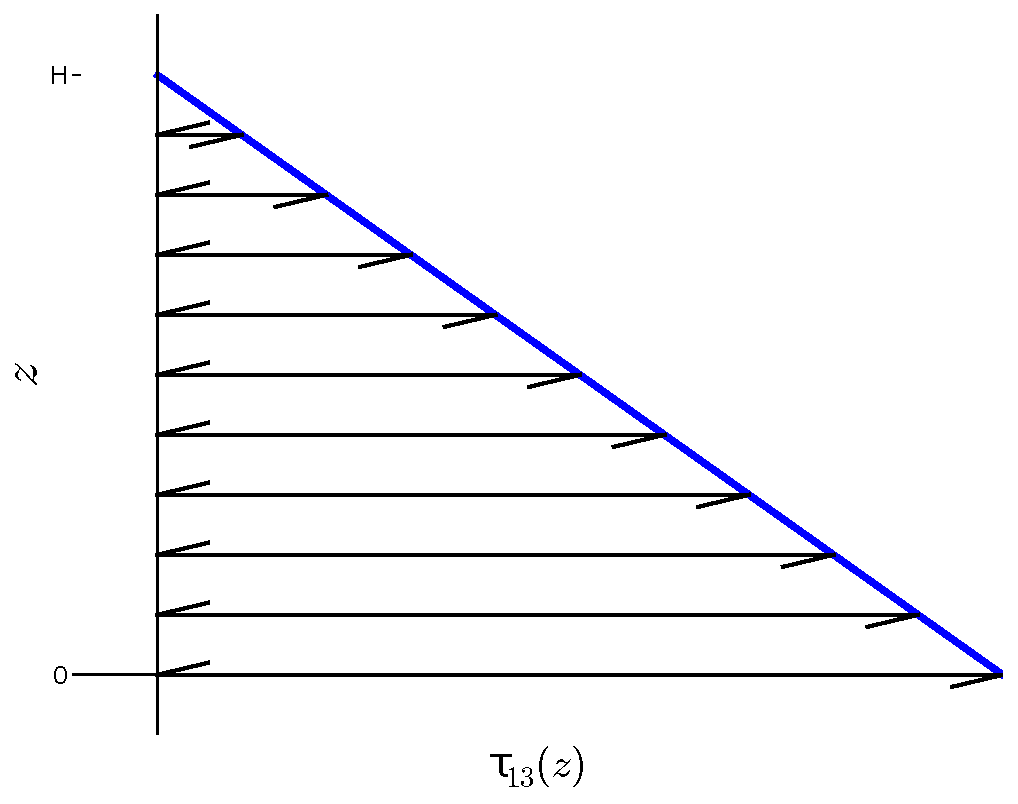
\includegraphics[width=0.4\textwidth]{slabshear}
\end{center}
\end{frame}


\begin{frame}{slab-on-a-slope 3}

\begin{columns}
\begin{column}{0.6\textwidth}
\begin{itemize}
\item do we believe these equations?
\item velocity on last slide (and below) was from a \emph{formula}
\item compare to observations at right
\end{itemize}
\begin{center}
% NOT preserving aspect ratio
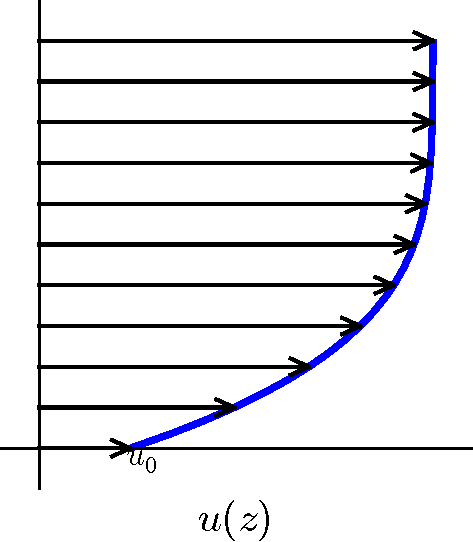
\includegraphics[width=0.6\textwidth,height=0.5\textheight]{slabvel}
\end{center}
\end{column}

\begin{column}{0.4\textwidth}
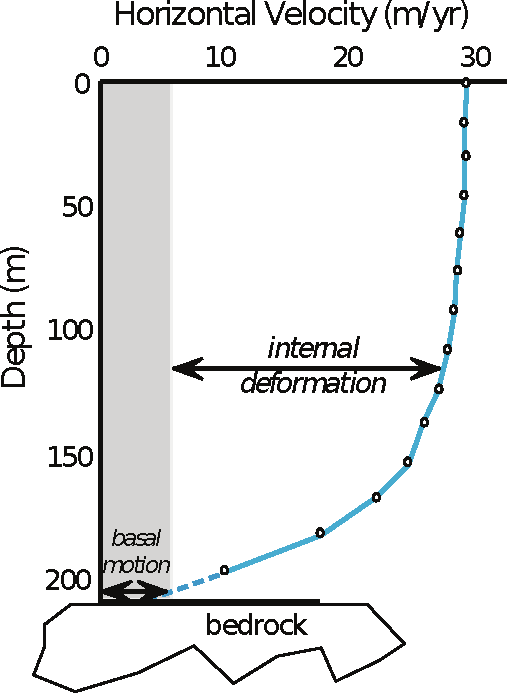
\includegraphics[width=1.0\textwidth]{athabasca_deform}

\medskip
\scriptsize
velocity profile of the Athabasca Glacier from inclinometry

\tiny (Savage and Paterson, 1963)
\end{column}
\end{columns}
\end{frame}


\begin{frame}{mass continuity}

\small
\begin{itemize}
\item now we know the velocity $u=u(t,x,z)$ \dots so what?
\item suppose our slab has variable thickness $H(t,x)$
\item compute the vertical average of velocity:
	$$\bar u(x,t) = \frac{1}{H}\int_0^{H} u(t,x,z)\,dz$$
\end{itemize}

\begin{columns}
\begin{column}{0.6\textwidth}
\begin{itemize}
\item consider change of area (ice volume in 3D) in the figure:
	$$\frac{dA}{dt} = \int_{x_1}^{x_2} M(x)\,dx + \bar u_1 H_1 - \bar u_2 H_2$$
\item but, assuming width $dx=x_2-x_1$ is small, $A\approx dx\, H$; divide by $dx$ and get
   $$H_t = M - \left(\bar u H\right)_x$$
\item this is a \emph{mass continuity equation}
\end{itemize}
\end{column}
\begin{column}{0.4\textwidth}
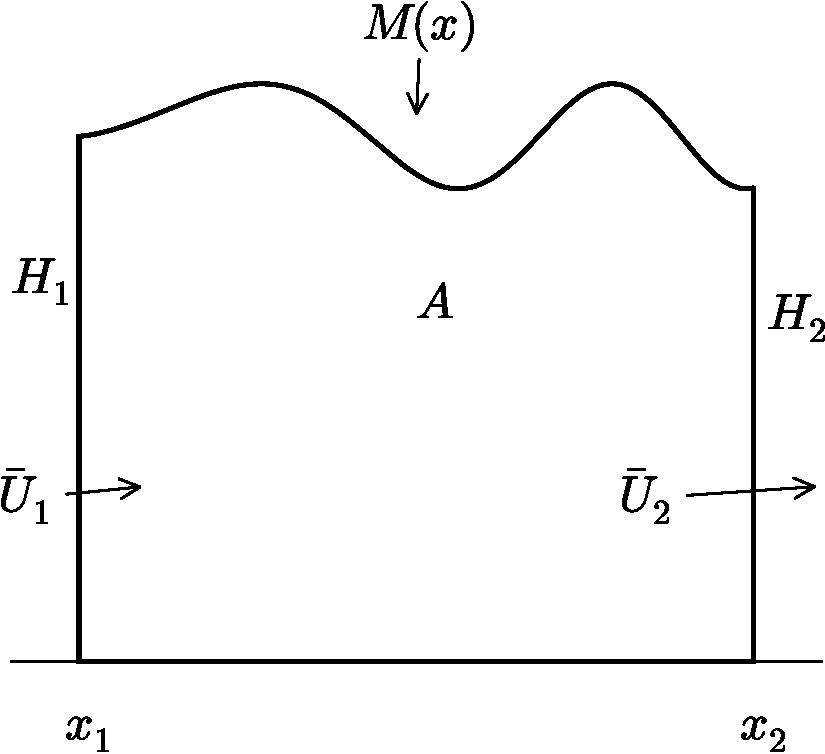
\includegraphics[width=1.0\textwidth]{slabmasscontfig}
\end{column}
\end{columns}
\end{frame}


\begin{frame}{rough explanation of ``shallow ice approximation'' (SIA)}

\small
\begin{itemize}
\item consider only $u_0=0$ case for now (``non-sliding SIA'')
\item from slab-on-slope velocity formula
\begin{align*}
\bar u H &= \int_0^H \frac{1}{2} A (\rho g \sin\alpha)^3  \left(H^4 - (H-z)^4\right)\,dz \\
	&= \frac{1}{2} A (\rho g \sin\alpha)^3  \left(\frac{4}{5} H^5\right) \\
	&= \frac{2}{5} A (\rho g \sin\alpha)^3 H^5
\end{align*}
\item note $\sin \alpha \approx \tan\alpha = - h_x$
\item combine with mass continuity $H_t = M - \left(\bar u H\right)_x$:
  $$H_t = M + \left(\frac{2}{5} (\rho g)^5 A H^5 |h_x|^2 h_x\right)_x.$$
\item this is SIA evolution equation for ice thickness
\item I'll return to this topic \dots
\end{itemize}
\end{frame}